\documentclass{Numerieke}
\newcommand\inv[1]{#1\raisebox{0.8ex}{$\scriptscriptstyle\!*$}}
\newcommand\transpose[1]{#1\raisebox{0.8ex}{$\scriptscriptstyle\!T$}}

%==PACKAGES==%
\usepackage[dutch]{babel}
\usepackage{graphicx}
\usepackage{float}
\usepackage{amsmath}
\usepackage{mathtools}
\usepackage[table,xcdraw]{xcolor}
\usepackage[normalem]{ulem}
\useunder{\uline}{\ul}{}
\graphicspath{{pictures/}}

\begin{document}
% == TITELPAGINA == %
%\input(nmbvoorblad)

%TEMP frontpage
\title{Numerieke Modellering en Benadering}
\maketitle

\section{QR factorisatie en kleinste kwadraten problemen}
\subsection{Opgave 1}
%==opgave==%
\textit{Wat zijn de eigenvectoren en bijhorende eigenwaarden van een 
	\textbf{Householder transformatiematrix?}
	Toon hoe je aan deze resultaten komt. Wat is de 
	\textbf{geometrische interpretatie}
	van deze waarden?
} \\
\newline
\textbf{1.A: Eigenwaarden en eigenvectoren} \newline
De vector $\vec{v}$ is een eigenvector van de vierkante matrix A \textit{(n$\times$n)} indien volgende vergelijking geldt:
 \[A\vec{v} = \lambda\vec{v}\] 
 Met $\lambda$  de bijhorende eigenwaarde en een natuurlijk getal.\newline 
 \newline
 \textit{Stelling:} \newline
 De Householder transformatie matrix F is orthogonaal en symmetrisch met enkel reeële waarden. \newline
 \textit{Bewijs: } \newline
 \textbf{F is symmetrisch} \newline
 \textit{Defenitie :} \(F=I-2\frac{v\inv{v}}{\inv{v}v}  \)
 \newline
 Met de genormaliseerde vector \(w = \frac{v}{\inv{v}v}\) is de defenitie herschrijfbaar als: 
 \[F=I-2w\inv{w}\]
 Aangezien de beide termen symmetrisch zijn is de householder transformatiematrix zelf ook symmetrisch.\newline
 \textbf{F is orthogonaal} \newline
 Indien \transpose{F}F=I zal F orthogonaal zijn.
 \[\transpose{F}F = \transpose{(I-2w\transpose{w})}(I-2w\transpose{w}) = (I-4w\transpose{w}+4w\transpose{w}w\transpose{w}) = I\]
 Hierbij is \transpose{w}w = 1 aangezien w genormaliseerd is. Daardoor wordt de vergelijking herleid tot : \newline
  \[\transpose{F}F = (I-4w\transpose{w}+4w\transpose{w}) = I\]
  \newline
 Aangezien F orthogonaal is, hebben de eigenwaarden een absolute waarde van 1 omdat de vermenigvuldiging met een orthogonale matrix een isometrie is.\newline
  F is symmetrisch en reeël dus alle eigenwaarden zullen reeël zijn. Daardoor kunnen de eigenwaarden kunnen herleidt worden tot 1 en -1.
  \newline
  Aangezien \(Fw = w-2w(\transpose{w}w)=-w}\) is minstens er één eigenwaarde -1 en voor alle vectoren u, loodrecht op w, geldt:  \(Fu = u-0w=u}\)
\newline
\newpage
\textbf{1.B: Geometrische interpretatie} \newline
\begin{figure}[H]
	\caption{Eigenwaarden en vectoren van de Householdertransformatiematrix}
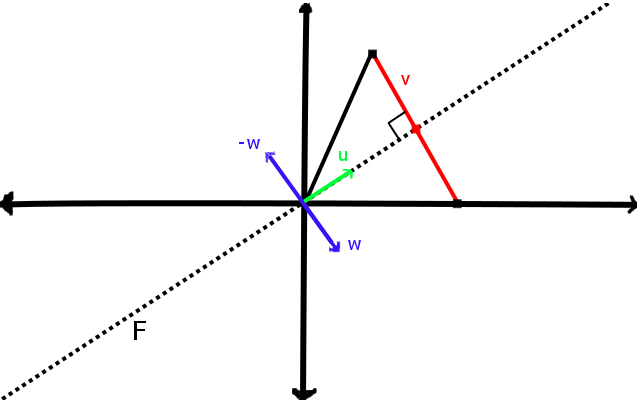
\includegraphics[scale=0.3]{Householdereigenwaarden.png}
\centering
\end{figure}
Zoals te zien is op de figuur zal de Householder functie de genormaliseerde vector w projecteren op -w omdat F een isometrie is. Daarnaast zullen alle loodrechte vectoren op w op F liggen en zals er geprojecteerd worden op hetzelfde punt.

\subsection{Opgave 2}
\textbf{2.B: Vergelijking resultaten}
% Please add the following required packages to your document preamble:
% \usepackage[table,xcdraw]{xcolor}
% If you use beamer only pass "xcolor=table" option, i.e. \documentclass[xcolor=table]{beamer}
% \usepackage[normalem]{ulem}
% \useunder{\uline}{\ul}{}
\begin{table}[H]
	\centering
	\caption{Conditie van A gelijk aan 1}
	\label{my-label}
	\begin{tabular}{l|
			>{\columncolor[HTML]{EFEFEF}}l 
			>{\columncolor[HTML]{EFEFEF}}l 
			>{\columncolor[HTML]{EFEFEF}}l 
			>{\columncolor[HTML]{EFEFEF}}l 
			>{\columncolor[HTML]{EFEFEF}}l 
			>{\columncolor[HTML]{EFEFEF}}l 
			>{\columncolor[HTML]{EFEFEF}}l 
			>{\columncolor[HTML]{EFEFEF}}l }
		\cline{2-9}
		\multicolumn{1}{c|}{{\ul \textbf{}}}               & \multicolumn{4}{c|}{\cellcolor[HTML]{C0C0C0}{\ul \textbf{Explicit}}}                                                                                                                                                                 & \multicolumn{4}{c|}{\cellcolor[HTML]{C0C0C0}{\ul \textbf{Implicit}}}                                                                                                                                                                 \\ \hline
		\multicolumn{1}{|l|}{\cellcolor[HTML]{C0C0C0}n}    & \multicolumn{1}{l|}{\cellcolor[HTML]{EFEFEF}\delta x} & \multicolumn{1}{l|}{\cellcolor[HTML]{EFEFEF}r} & \multicolumn{1}{l|}{\cellcolor[HTML]{EFEFEF}\delta x/x} & \multicolumn{1}{l|}{\cellcolor[HTML]{EFEFEF}K(A)r/b} & \multicolumn{1}{l|}{\cellcolor[HTML]{EFEFEF}\delta x} & \multicolumn{1}{l|}{\cellcolor[HTML]{EFEFEF}r} & \multicolumn{1}{l|}{\cellcolor[HTML]{EFEFEF}\delta x/x} & \multicolumn{1}{l|}{\cellcolor[HTML]{EFEFEF}K(A)r/b} \\ \hline
	\multicolumn{1}{|l|}{\cellcolor[HTML]{C0C0C0}10}   & 6.9162e-16                                          & 6.2979e-16                                         & 4.1395e-16                                                & 3.7762e-16                                                    & 5.9923e-16                                          & 6.5433e-16                                         & 3.6326e-16                                                & 3.9842e-16                                                    \\ \cline{1-1}
	\multicolumn{1}{|l|}{\cellcolor[HTML]{C0C0C0}100}  & 1.5897e-14                                          & 1.6162e-14                                         & 3.0763e-15                                                & 3.099e-15                                                     & 6.4763e-15                                          & 6.3391e-15                                         & 1.3988e-15                                                & 1.3992e-15                                                    \\ \cline{1-1}
	\multicolumn{1}{|l|}{\cellcolor[HTML]{C0C0C0}1000} & 2.6441e-13                                          & 2.6477e-13                                         & 1.6695e-14                                                & 1.6723e-14                                                    & 4.9441e-14                                          & 4.93e-14                                           & 3.7536e-15                                                & 3.7537e-15                                                    \\ \cline{1-1}
\end{tabular}
\end{table}
 \begin{table}[H]
 	\centering
 	\caption{Conditie van A gelijk aan 10^4}
 	\label{my-label}
 	\begin{tabular}{l|
 			>{\columncolor[HTML]{EFEFEF}}l 
 			>{\columncolor[HTML]{EFEFEF}}l 
 			>{\columncolor[HTML]{EFEFEF}}l 
 			>{\columncolor[HTML]{EFEFEF}}l 
 			>{\columncolor[HTML]{EFEFEF}}l 
 			>{\columncolor[HTML]{EFEFEF}}l 
 			>{\columncolor[HTML]{EFEFEF}}l 
 			>{\columncolor[HTML]{EFEFEF}}l }
 		\cline{2-9}
 		\multicolumn{1}{c|}{{\ul \textbf{}}}               & \multicolumn{4}{c|}{\cellcolor[HTML]{C0C0C0}{\ul \textbf{Explicit}}}                                                                                                                                                                 & \multicolumn{4}{c|}{\cellcolor[HTML]{C0C0C0}{\ul \textbf{Implicit}}}                                                                                                                                                                 \\ \hline
 		\multicolumn{1}{|l|}{\cellcolor[HTML]{C0C0C0}n}    & \multicolumn{1}{l|}{\cellcolor[HTML]{EFEFEF}\delta x} & \multicolumn{1}{l|}{\cellcolor[HTML]{EFEFEF}r} & \multicolumn{1}{l|}{\cellcolor[HTML]{EFEFEF}\delta x/x} & \multicolumn{1}{l|}{\cellcolor[HTML]{EFEFEF}K(A)r/b} & \multicolumn{1}{l|}{\cellcolor[HTML]{EFEFEF}\delta x} & \multicolumn{1}{l|}{\cellcolor[HTML]{EFEFEF}r} & \multicolumn{1}{l|}{\cellcolor[HTML]{EFEFEF}\delta x/x} & \multicolumn{1}{l|}{\cellcolor[HTML]{EFEFEF}K(A)r/b} \\ \hline
	 	\multicolumn{1}{|l|}{\cellcolor[HTML]{C0C0C0}10}   & 3.0736e-12                                          & 6.4259e-12                                         & 1.8003e-12                                                & 4.5603e-12                                                    & 1.722e-12                                           & 3.3718e-12                                         & 1.0098e-12                                                & 2.3895e-12                                                    \\ \cline{1-1}
	 	\multicolumn{1}{|l|}{\cellcolor[HTML]{C0C0C0}100}  & 9.2189e-11                                          & 9.7262e-11                                         & 1.6467e-11                                                & 2.2014e-11                                                    & 1.8454e-11                                          & 2.7045e-11                                         & 3.7652e-12                                                & 6.9365e-12                                                    \\ \cline{1-1}
	 	\multicolumn{1}{|l|}{\cellcolor[HTML]{C0C0C0}1000} & 1.5252e-09                                          & 1.533e-09                                          & 9.5391e-11                                                & 1.1298e-10                                                    & 1.6481e-10                                          & 1.7583e-10                                         & 1.1824e-11                                                & 1.636e-11                                                     \\ \cline{1-1}
	 \end{tabular}
 \end{table}
 \begin{table}[H]
 	\centering
 	\caption{Conditie van A gelijk aan 10^8}
 	\label{my-label}
 	\begin{tabular}{l|
 			>{\columncolor[HTML]{EFEFEF}}l 
 			>{\columncolor[HTML]{EFEFEF}}l 
 			>{\columncolor[HTML]{EFEFEF}}l 
 			>{\columncolor[HTML]{EFEFEF}}l 
 			>{\columncolor[HTML]{EFEFEF}}l 
 			>{\columncolor[HTML]{EFEFEF}}l 
 			>{\columncolor[HTML]{EFEFEF}}l 
 			>{\columncolor[HTML]{EFEFEF}}l }
 		\cline{2-9}
 		\multicolumn{1}{c|}{{\ul \textbf{}}}               & \multicolumn{4}{c|}{\cellcolor[HTML]{C0C0C0}{\ul \textbf{Explicit}}}                                                                                                                                                                 & \multicolumn{4}{c|}{\cellcolor[HTML]{C0C0C0}{\ul \textbf{Implicit}}}                                                                                                                                                                 \\ \hline
 		\multicolumn{1}{|l|}{\cellcolor[HTML]{C0C0C0}n}    & \multicolumn{1}{l|}{\cellcolor[HTML]{EFEFEF}\delta x} & \multicolumn{1}{l|}{\cellcolor[HTML]{EFEFEF}r} & \multicolumn{1}{l|}{\cellcolor[HTML]{EFEFEF}\delta x/x} & \multicolumn{1}{l|}{\cellcolor[HTML]{EFEFEF}K(A)r/b} & \multicolumn{1}{l|}{\cellcolor[HTML]{EFEFEF}\delta x} & \multicolumn{1}{l|}{\cellcolor[HTML]{EFEFEF}r} & \multicolumn{1}{l|}{\cellcolor[HTML]{EFEFEF}\delta x/x} & \multicolumn{1}{l|}{\cellcolor[HTML]{EFEFEF}K(A)r/b} \\ \hline
		\multicolumn{1}{|l|}{\cellcolor[HTML]{C0C0C0}10}   & 2.7567e-08                                          & 4.432e-08                                              & 1.6671e-08                                                & 3.499e-08                                                     & 1.6694e-08                                          & 2.4974e-08                                             & 9.8794e-09                                                & 1.785e-08                                                     \\ \cline{1-1}
		\multicolumn{1}{|l|}{\cellcolor[HTML]{C0C0C0}100}  & 8.0343e-07                                          & 8.27904e-07                                            & 1.5567e-07                                                & 1.9718e-07                                                    & 1.4431e-07                                          & 1.78499e-07                                            & 3.2706e-08                                                & 4.9677e-08                                                  \\ \cline{1-1}
		\multicolumn{1}{|l|}{\cellcolor[HTML]{C0C0C0}1000} & 1.533e-05                                           & 1.542e-05                                         & 9.5357e-07                                                & 1.1203e-06                                                    & 1.526e-06                                           & 1.6375e-06                                           & 1.086e-07                                                 & 1.4195e-07                                                    \\ \cline{1-1}
	\end{tabular}
\end{table}

TODO : Meer Verklaren \newline
\newline
Bij het vergelijken van de impliciete en expliciete methoden voor matrices van dezelfde grootte is er een klein verschil in nauwkeurigheid. De Impliciete functie zal iets nauwkeuriger zijn omdat het de matrix Q zelf niet meer moet samenstellen en zo minder onderhevig zijn aan afrondingsfouten. Verder is het zichtbaar dat voor alle conditiegetallen van A de nauwkeurigheid van de resultaten zal dalen naarmate de grootte van A toeneemt. Dit komt omdat er meer elementen van x berekend moeten worden en daardoor meer fouten in het algoritme kunnen voorkomen. \newline
De scherpte van de grens blijft ongeveer hetzelfde voor de verschillende condities van A.  
\begin{figure}[H]
	\caption{Uitvoeringstijd: Expliciet(rood), Impliciet(Blauw) }
	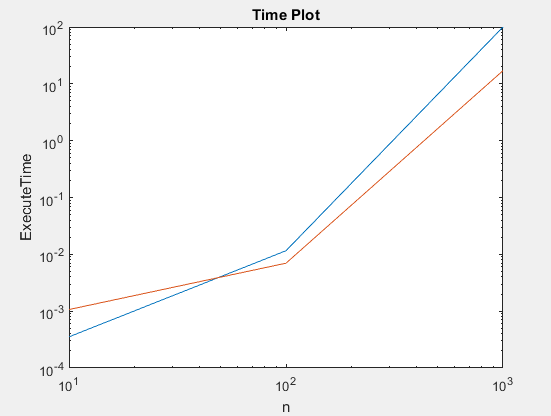
\includegraphics[scale=0.6]{HouseholderTimePlot.png}
	\centering
\end{figure}
TODO: niet zeker \newline
\newline
In het algemeen geval zou de impliciete versie sneller moeten zijn als de expliciete versie. In opdracht 2 is dit enkel het geval bij de kleine matrix. Dit komt omdat we gebruik maken van 2 scripts die elk een for lus gebruiken over de groote van de matrix terwijl dit bij de expliciete versie maar 1 is. Verder heeft de conditie van de matrix geen invloed op de uitvoeringstijd van beide algoritmes. 

\subsection{Opgave 3}
Met behulp van de QR factorisatie is het mogelijk om een kleinste kwadraten probleem op te lossen. De projector \(P=Q\inv{Q}\) projecteert de vector b in de range van A en zo is het mogelijk om een exacte oplossing van x te vinden voor \(QRx=Q\inv{Q}\). Dit zal dan herleidt worden tot \(Rx=Qb\) en zal de uitkomst zo dicht mogelijk bij de waarden van b liggen. 
\begin{figure}[H]
	\centering
	\caption{Vergelijking tijdsvertragingen}
	\begin{minipage}[l]{.3\textwidth}
		\centering
		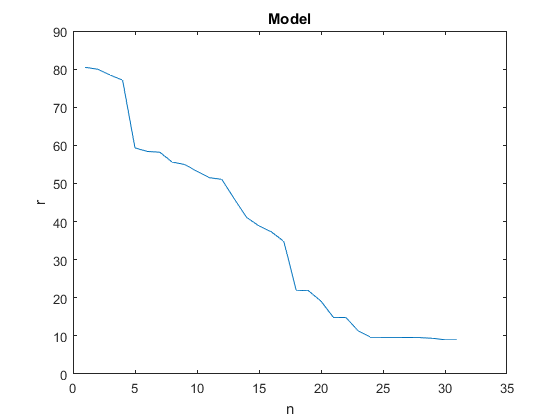
\includegraphics[width=1.1\linewidth]{Model_opgave3}
		\captionof{Residu}
		\label{fig:test1}
	\end{minipage}%
	\begin{minipage}[r]{.3\textwidth}
		\centering
		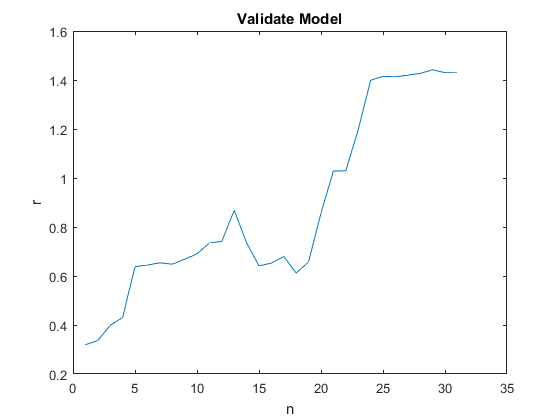
\includegraphics[width=1.1\linewidth]{Validate_model_opgave3}
		\captionof{Validate model}
		\label{fig:test2}
	\end{minipage}
\end{figure}
Bij de lage tijdsvertraging zal het residu en de fout met het de data in validate.mat het kleinste zijn dus een kleine n zal een geschikte keuze zijn.




\end{document}